\section{Related Work}

Many authors investigated on IoT cloud computing and emphasize its potential to improve efficiency and reduce costs in IoT because computing resources can be scaled and virtualized in a flexible manner. \citeauthor{laghari2021review} in their \textit{Review and State of Art of Internet of Things} point out the tight interconnection between cloud and IoT and they emphasize advantages that the intermingling of IoT and cloud have. \citeauthor{almolhis2020security} attest the beneficial characteristics of cloud computing in IoT technologies in terms of on-demand self-service, resource pooling, broad network, measured service, and rapid elasticity. However, the large part of literature agrees repeatedly on criticalities of the cloud IoT, like security, data ownership, potential crashes and latency and \citeauthor{almolhis2020security} recommend to put immediate attention in the research community especially on open security topics.

\begin{figure}[htbp]
\centerline{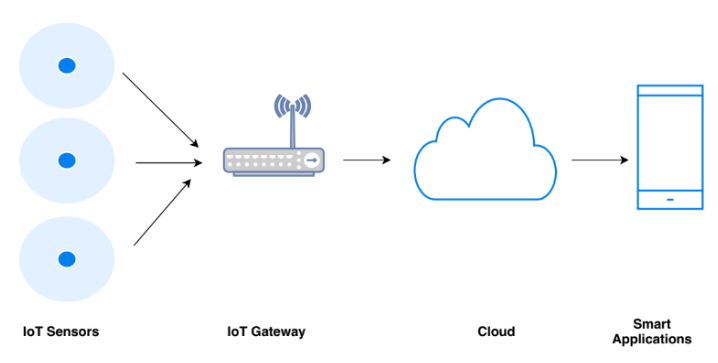
\includegraphics[scale=0.35]{images/iot_cloud_application_scenario.png}}
\caption{Sample of IoT cloud application scenario by \citeauthor{almolhis2020security}}
\label{fig}
\end{figure}

In the context of smart grids, the term \textit{hybrid-cloud usage} appears frequently and seems to be clearly favoured over "cloud-only" approaches for several reasons. \citeauthor{talaat2020hybrid} for example suggest to integrate data processing hardware devices to a private cloud to overcome security issues in the public cloud. \citeauthor{zahoor2018cloudmanag} recommend cloud-fog-based smart grid model for efficient resource management \cite{zahoor2018cloudmanag} and utilization \cite{zahoor2018cloudutil}. They explain how the amount of transmitted data and data transmission time can be significantly reduced because the fog approach reduces the amounts of data transmitted to the cloud by performing decentralized data processing. It means that some of the processing units and storage is placed closer to where data is actually being sourced from. It can furthermore address security issues and certain regulations (e.g. in relation to data ownership).

\citeauthor{7396147} investigate in how IoT systems' governance can be improved in terms of uncertainty in the system infrastructure. Uncertainty can be caused by many reasons, e.g. probe failures, network issues or human error and puts a lot of burden on the developers and operation mangagers (users) when managing runtime governance in IoT cloud systems \cite{7396147}. But it is a big challenge to include uncertainties in the development of proper governance strategies. \citeauthor{7396147} introduce the U-GovOps framework for \textit{dynamic, on-demand governance of elastic IoT cloud systems under uncertainty}. It consists of a declarative policy language that basically allows the developers to model uncertainties for their governance strategies and mechanisms that support the execution of the strategies taking the modeled uncertainties into account.

\citeauthor{bornhoft2013simulation} showed with a simulation model of a smart grid integration into an office building how much energy costs could be saved if the energy consumption was steered by taking a hypothetical dynamic price model into account. Depending on the current supply and demand of electricity, they reduced consumption or increased the amount energy stored in thermal energy storages. In their model, they could economize up to 31\% of their usual energy costs by optimizing the energy consumption depending on the current price of electricity.

Zurich has a test area called \textit{Greencity}, where the electricity utility of Zurich (ewz) maintains a pilot project in form of an integral energy infrastructure with intelligent power regulation mechanisms. \citeauthor{baumgartner2020monitoring} summarize findings about the \textit{monitoring concept suitable for utilising flexibilities in the low-voltage distribution grid in Greencity}. Their main focus was to gain experience with cloud architecture in terms of processing data collected by sensors. In the case of \textit{Greencity}, field data is streamed into a Microsoft Azure cloud computing environment for processing. They also seize on security and data protection issues in the context of using a cloud provider for hosting their services, but state that for their use case the Azure cloud architecture fulfils the information security requirements and for data protection they set up individual load profiles.

Testbeds represent a common experimentation platform where (prototypical) IoT devices or applications can be deployed and verified. According to \citeauthor{cintuglu2016cloud}, traditional testbeds tend to cover a limited project frame, while complex IoT systems, like smart grids, due to their interdisciplinary structure, require multiple heterogeneous test environments with different capabilities to interconnect in real-time. They therefore claim on more complete test platforms for comprehensive system testing and propose to include cloud communication for testbed implementation. They design a cloud-enabled architecture, where they outline the most relevant aspects how this can be achieved. Their proposal of a cloud enabled remote access smart grid testbed platform was implemented by the Energy Systems Research Laboratory, Florida International University.


